
%Mise en page
\documentclass[12pt]{article}   % Indique que ce document est de type 'article', avec une page titre
%\usepackage{natbib}
\usepackage[letterpaper,margin=1in]{geometry}    % Élargir les marges
\usepackage{fancyhdr}
\pagestyle{fancy}
\usepackage{setspace}      % Double inerligne
\usepackage{rotating}      % Avoir des pages horizontale
\usepackage[toc,page]{appendix}    % Créer un appendix
\usepackage[nottoc]{tocbibind}
\usepackage{amsmath}
% L'écriture en français
\usepackage[T1]{fontenc}     % Le PDF supporte les caractères accentués
\usepackage[utf8]{inputenc}     % Encodage UTF-8, supporte les caractères accentués
\usepackage{titlesec}      % Title seperation
\usepackage{csquotes}

% Science
\usepackage{amsmath, amsfonts, amsthm,mathtools}  % Tout pour algébrer 'LES MATHS'
\usepackage{chemist}       % Pour les formules chimiques
\usepackage{color}       % Pour les couleurs dans le code source
\usepackage{listings}      % Écrire des codes sources
\DeclarePairedDelimiter\abs{\lvert}{\rvert}%
\DeclarePairedDelimiter\norm{\lVert}{\rVert}%

%Graphique et tableaux
\usepackage{float}       % Graphiques et figures
\usepackage{graphicx}      % Pour inclure le code source en annexe
\usepackage[section]{placeins}     % Pour les graph comme du monde
\usepackage{multirow}       % tableau multiple
\usepackage{tabulary}      % tableau avec case en Y auto
\usepackage{tikz}        % image en tikz
\usepackage{pgfplots}       % graphique en .pdf
\usepackage{pgfgantt}      % ???
\pgfplotsset{compat=newest}
\pgfplotsset{plot coordinates/math parser=false}

% Outils divers
\usepackage{comment}      % pour les commentaires
\usepackage{pdflscape}       % mettre la page vertical
\usepackage{adjustbox,lipsum}     % ajuste les boites
\usepackage{array}
\usepackage{dashrule}
\usepackage{booktabs}


 % Special FRQNT setting
\usepackage{biblatex} % references: https://www.overleaf.com/learn/latex/Bibliography_management_in_LaTeX
\addbibresource{ref.bib}
\defbibheading{bibliography}{\textbf{References}}
\lhead{Dynamique et modélisation des innondations estuariennes}
\rhead{Beaudoin, Jean-François}
\renewcommand{\headrulewidth}{0pt}
\titlespacing*{\section}{0pt}{1.5ex plus 1ex minus .2ex}{0.7ex plus .2ex}
\titleformat*{\section}{\large\bfseries}
\setlength{\parindent}{3em}
\setlength{\parskip}{1em}

%\setlength{\bibsep}{0.1pt}
\doublespacing
\begin{document}

%-------------------------------
%	TITLE SECTION (do not modify unless you really need to)
%-------------------------------
%\fancyhead[C]{}
\hrule \medskip
\begin{minipage}{0.295\textwidth} 
\raggedright
\footnotesize
\yourname \hfill
\end{minipage}
\begin{minipage}{0.4\textwidth} 
\centering 
\large 
Revue de littérature sur les différentes méthode de cartographie des innondations et de l'étude de l'hydrodynamique des estuaires.
\normalsize 
\end{minipage}
\begin{minipage}{0.295\textwidth} 
\raggedleft
\today\hfill\\
\end{minipage}
\medskip\hrule 
\bigskip


%-------------------------------
%	ASSIGNMENT CONTENT (add your responses)
%-------------------------------%------------------------------------------------
\section{Introduction} % this is an example

Les deltas et les estuaires sont des millieux où les innondations sont causées par l'interaction entre des phénomènes océanographiques, hydrologiques et météorologiques. Ils sont à la fois vulnérables au phénomène d'innondations côtières et aux phénomènes d'innondations fluviales. Ce sont des endroits potentiellement vulnérable à ce qu'on appelle des catastrophes conjointes.
\par
Selon le GIEC les catastrophes conjointes sont définis comme: (1) deux événements extrêmes ou plus qui arrive en même temps ou en succession rapide. (2) La combinaison d'événements extrêmes avec des conditions de bases qui amplifie l'impact de l'aléa ou, (3) Une combinaisons d'événement qui ne sont pas extrême mais dont les impacts combinés sont extrêmes.\cite{Lal2012} 
\par
Les catastrophes conjointes ont lieux lorsque deux événement ayant une relation statistique significative interagissent ensemble ou s'ils ont lieu en succession rapide empirant ainsi les conséquences de chacunes d'entre elles. Par exemple, plusiseurs feux de forêt simultanées, une secheresse suivi d'un feu de brousse ou encore deux tempêtes tropicales successives. Tout ces évênement simultanée ou en succession rapides empire les conséquences des événements individuels. \cite{Leonard2014} 
\par
Dans les estuaires, les innondations composés ont lieu lorsque les crues et les ondes de tempêtes interagissent constructivement pour augmenter le niveau d'eau. Il pose des problèmes particuliers en ce qui concerne la gestion des risques  \cite{Zscheischler2018}. Environ 1.5$\%$ des innondations en europe sont des événement conjoints entre 1870 et 2016 \cite{Paprotny2018b}.  La sensibilité des estuaires et les risques d'inondations dépendent de plusieurs facteurs, principalement liés aux caractéristiques géomorphologiques du territoire (Géométrie de l'estuaire, type de sédiments, régime hydrologique, etc). Ce sont donc des endroits où l'évaluation et la gestion du risque nécéssite une plus grande attention.
\par
Le problème des innondations estuariennes (et des catastrophes naturelles en générales) se situe à deux niveaux. Il faut savoir à la fois la probabilité qu'un évênement se produise et les conséquences potentielles pour bien évaluer et gêrer le risque.
\par
Les risques pour les citoyens habitant le long des cours d'eau peuvent être déterminés par des modèles d'innondations. Ces modèles permettent de définir les zones à risque et des indices de danger sur le territoire.
\par
Dans un estuaire, la dynamique des innondations n'est pas la même que pour une innondation dans la plaine alluvial ou celle d'une innondation côtière qui sont tout les deux forcé par un seul mécanisme. Les ondes de marées et les ondes de crues interagissent ensemble ce qui modifie les courants et crée des mécanismes d'innondation suplémentaires comme du refoulement. Physiquement, la propagation de l'ondes de marées, des vagues et de la crues dépendent de la géométrie du bassin. Ainsi, pour bien évaluer les risques d'innondation à un endroit précis les modèles hydrodynamique permettent beaucoup de flexibilité et une fois bien calibrer ils permettent de simuler ces interactions. À partir d'événements connus, il sera alors possible de définir des zones à risques et faire des études de sensibilité du système. La première partie de cette revue de littérature s'interessera donc aux différentes méthodologies de modélisation pour la réalisation de cartes d'innondations. Il y aura une présentation des différents modèles hydrodynamiques et des différentes études de cas appliqué à différents estuaires. 
\par
Les modèles hydrodynamiques permettent donc de comprendre quels sont les conséquences d'un événement conjoint. Ces derniers permettent d'identifier les endroits à risque selon des conditions extrêmes définis par le modélisateur. Pour obtenir une évaluation complètes des risques associés aux innondations estuariennes, il faut aussi faire une analyse des statistiques d'innondations à l'embouchure des rivières. En effet, pour bien évaluer les risques, il faut comprendre la physique des innondations, mais il faut aussi comprendre la probabilités que ces innondations surviennent. Pour cela, il faut utiliser les copules pour trouver la distribution de probabilité conjointe des crues et des onde de tempête. L'analyses de copules permet aussi de calculer des périodes de retour d'événement extrême. La deuxième partie de la revue de littérature fera donc un résumé des connaissances et de l'utilisation des copules pour modéliser les probabilités d'un événement conjoint dans le contexte des innondations estuariennes.  

\section{Modélisation des innondations estuarienne}

Il existe 2 grand type de modèles d'inondations qui permettent de produire des cartes d'inondations et de prédire les risques futures \cite{Teng2017}. Les modèles empiriques et les modèles hydrodynamiques.
    
\subsection{modèles empiriques}

Les modèles empiriques utilise des données terrains (observation) obtenues de diverse façon afin de comprendre l'historique d'innondations d'un endroits en particulier. Ce type de modèle se fie sur le passé pour tenter de prédire l'avenir et nécéssite une certaine quantités de données terrains pour pouvoir être juste. Les modèles empiriques peuvent par la suite être utilisés pour valider les modèles hydrodynamiques.

\subsection{modèle 1D}
  
  Afin de bien comprendre et de prédire les différents processus qui cause les innondations fluviales, différents type de modèles hydrodynamique correspondant à différents niveau de simplification des équations de la dynamiques des fluides sont utilisés. Il existe des modèles à une dimension. Par exemple, HEC-RAS ou la SOBEK Suite de deltares ont des modules de modélisation en une dimension. 
  
  Le modèle HEC-RAS peut résoudre différentes équations en une dimension. Pour ce modèles, l'équation de la différence de hauteur d'eau entre 2 section transversales est donné par: 
    
    \begin{align}
        Z_2 +Y_2+\frac{A_2 V_2^2}{2g} = Z_1 +Y_1+\frac{A_1 V_1^2}{2g}+ h_e
    \end{align}
    
    Où : 
    \begin{align}
     Z_1,Z_2 = \textit{Hauteur du terrain le long du chenal principale}\\
     Y_1,Y_2 = \textit{Profondeur de l'eau aux sections transversales le long du chenal}\\
     V_1,V_2 = \textit{Vitesse moyenne (Débit/aire de l'écoulement)}\\
     a_1,a_2 = \textit{Pondération de la vitesse}\\
     g = 9.8 m/s^2\\
     h_e = \textit{Perte de charge d'énergie} 
    \end{align}
    
    Le modèle calcul donc un pente moyenne selon la géométrie de l'écoulement et un coefficient de perte de charge qui correspond à la friction et à la contraction de l'écoulement. 
    
    Il s'agit d'une équation statique qui calcule la hauteur d'eau en fonction de la pente du terrain et qui calcul la vitesse avec l'aire de l'écoulement le long de section transversales. Cette équation très simplifié a l'avantage d'être très rapide à calculer. Elle permet donc de faire des statistiques avec un grand nombre de simulations. Cependant elle ne prend pas en compte l'évolution temporelle de l'onde de crues. Elle ne prends pas non plus en compte le passage d'un écoulement critique à un écoulement sous-critique. Considérant les conditions frontières complexe à l'embouchure des rivière et la complexité spatio-temporelle d'une circulation estuarienne cette équation ne permet pas de bien représenter les effets d'une onde de marée dans le système fluviale.
    
    Toujours en une dimension, il est possible de résoudre des systèmes dynamiques en utilisant les équations de St-Venant à une dimension qui s'écrivent comme:
    
    \begin{align}
       \text{Conservation de la masse \quad}  \dfrac{\partial Q}{\partial x} + \dfrac{\partial A}{\partial t} = 0 
    \end{align}
    \begin{align}
       \textit{Conservation de la quantité de mouvement \quad}  \frac{1}{A}\frac{\partial Q}{\partial t} + \frac{1}{A}\frac{ \partial \frac{Q^2}{A}}{\partial x} + g \frac{\partial h }{\partial x} - g(S_o - S_f) = 0 
       \label{stevnant}
    \end{align}
    
    Cette équation (qui peut être écrit sous d'autres formes) permet elle aussi d'être résolue rapidement et d'utiliser comme conditions frontières en amont des histogramme de crues qui varie dans le temps afin d'avoir des séries temporelles de hauteur d'eau à chaques sections transversales. Par contre, ces modèles ne calculent pas la dynamique complexes des transport latéral de masse d'eau sur la plaine inondables et la topographie est nécéssairement approximé de façon discrète entre les section transversales. Ainsi, ces modèles sont moins adapté pour obtenir les vitesses de courant ou faire de la modélisation précise dans des contexte ou l'hydrodynamique est complexe. Cependant, ils sont très utiles dans les cas où il faut faire des statistiques sur de longues séries temporelles ou pour faire des études statistiques sur de nombreuses simulations. 
    
    Ils sont aussi utilies pour sauver du temps en couplant des modèles 1D et 2D ensemble. En effet, les modèles 1D sont approprié pour résoudre les innondations dans les chenaux où les variations spatiales des vitesse sont plus petites. Dans la plaine alluvial un modèle 2D peut être couplé ce qui sauve du temps de calcul tout en permettant des prédictions précises de l'innondation.\cite{Liu2015}
    
    \subsection{modèles 2D}
    
    Les modèles hydrodynamiques 2D sont présentement les plus utilisées principalement grâce à leurs flexibilité et leur relative simplicité conceptuelle. De façon générale, ces modèles résolve les équations de navier stokes avec l'approximation en eau peu profonde.
    
    Il y a alors deux équation du momemtum (une pour chaque dimension) et une équation de conservation de la masse.
    
    \begin{align}
        \textit{Conservation de la masse \quad} \frac{\partial h}{\partial t} + \frac{ \partial hu}{\partial x} + \frac{ \partial hv}{\partial y} + q  = 0 
        \label{masse2d}
    \end{align}
    
     \begin{align}
       \textit{Conservation de la quantité de mouvement \quad}\\
       \frac{\partial\Vec{v}}{\partial t} + \Vec{v}\cdot \nabla\Vec{v} = -g\nabla h + \nu_t \nabla^2 \Vec{v} + c_f  \Vec{v} + f\Vec{k}\times v
    \end{align}
    
    Il existe aussi des modèles dit à deux trois termes qui néglige certain terme dans l'équation en eau peu profondes. 
    
    Par exemple, pour un écoulement à l'équilibre hydrodynamique où la gravité est compensé par la friction, les termes de dépendance temporelle, d'advection, de viscosité turbulentes et de coriolis peuvent être négligé. L'équation s'écrit alors comme:
    
    \begin{align}
        g\nabla h = c_f  \Vec{v}
        \label{onde1}
    \end{align}
    
    En utilisant la formulation de manning pour le coeficient de friction:
    
    \begin{align}
        c_f = \frac{n^2 g \abs{v}}{R^{4/3}}
    \end{align}
    
    On peut réécrire l'équation \ref{onde1} de la quantité de mouvement comme:
    
    \begin{align}
     g\nabla h = \frac{n^2 g \abs{v}}{R^{4/3}}\Vec{v} 
    \end{align}
    
    Qui devient après quelques simplification:
    
     \begin{align}
     V = \frac{-R^{2/3}}{n}\frac{\nabla h}{[\abs{\nabla h}]^{1/2}}
     \label{vonde}
    \end{align}
    
    Par la suite, on substitue \ref{vonde} dans \ref{masse2d} pour obtenir l'équation de diffusion d'onde. Il s'agit d'une équaton différentiel qui permet de trouver la hauteur d'eau dans le temps en fonction en fonction de la friction au fond et de la différence de hauteur d'eau entre deux points de grille. 
    
        \begin{align}
     \frac{\partial H}{\partial t} - \nabla \cdot \frac{-R^{5/3}}{n [\abs{\nabla h}]^{1/2}} \nabla h + q = 0 
    \end{align}
    
     HEC-RAS permet la résolution de cette équation de diffusion d'onde pour résoudre les niveaux d'eau sur un domaine en deux dimension. C'est aussi ce type d'équation qu'utilise le modèle LISFLOOD-FP (\cite{BATES201033}). Ce dernier est un modèle dit à trois termes qui néglige l'advection dans les équations. Selon, \cite{Hunter2007} les résultats de ces modèles sont valables lorsque les vitesses sont faibles. Ceux-ci peuvent donc être inadéquat dans le cas d'une innondation urbaine ou les vitesses de courants sont plus forte et les profondeurs moins élevées. 
    
    \subsection{modèle 3D}
    
    Les modèles 3D sont particulièrement interessant pour ce qui concerne les écoulements où la structure varie rapidement dans l'espace ou dans le temps. Par exemple, les inondations causé par des ruptures de barrage, des tsunamis et la ruptures de digue.\cite{Teng2017} Les modèles 3D résolvent les équations de Navier-stokes complètes pour un fluide incompressible:
    
    \begin{align}
        \textit{Conservation de la quantité de mouvement \quad} \frac{\partial u}{\partial t} + u\cdot \nabla u + \frac{1}{\rho} \nabla p = g + \mu \nabla^2 u
    \end{align}
    
    Ces modèles permettent aussi de résoudre les effets de la dynamique provenant des gradients de densité des écoulements tri-dimensionnelle comme les instabilités baroclines et le mélange qui ont un impact important sur la dynamique à  Sous-méso-échelle (1-20km). 
    
    \subsection{modèle 0D}
    
    Enfin, des modèles hydrodynamiques très simplifié permettent aussi d'estimer les risques d'innondations. Des modèles de type "bathub" transfère l'eau partout où le niveau de la terre est en bas du niveau de l'eau s'il existe une connection hydrologique entre les cellules du modèle. Ce sont des modèles à 0 dimensions car l'hydrodynamique n'est pas résolu. Ces modèles peuvent être implémenté directement dans un GIS et sont extrêmement efficace. Il ne prenne en compte ny la dynamique du transport latéral ni les pertes d'énergie du à la friction. Cela revient à faire l'approximation que le pic de crues a lieu indéfiniment dans le système.
    
    \section{Applications aux estuaires}
    
    Les modèles hydrodynamique permettent une grande flexibilité dans les applications scientifiques et les possibilités de méthodologies sont nombreuses. Chaque modèle a des forces et des faiblesses et plusieurs études de cas sur différents estuaires ont été menés. Certaines de ces études sont des études de la dynamique estuarienne,\cite{Twigt2009,Spearman1998, Yang2012, Hein2011,Du2018, Kumbier20182} . D'autres tente de simuler des événement d'innondation réelles afin de construire des modèles d'innondation hydrodynamique \cite{Lee2019, martyr2013, Kumbier2019, Kumbier2018}.  

    \subsection{Modèle 1D}

    La complexité de l'interaction entre les ondes de marées et l'ondes de crues font en sorte que les modèles 1D sont moins bien adaptés pour résoudre une innondation en zone estuarienne \cite{Teng2017}. Cependant, l'efficacité en termes de ressource de calculs de ces modèles font en sorte qu'ils ont été utilisé par le passé. Ils sont utiles dans le cadre d'un couplage 1D-2D pour sauver du temps de calcul sur un domaine où les complexités hydrodynamiques sont localisé dans l'espace. C'est lorsque le temps de calcul est un élément important à prendre en compte qu'il sont utiles.
    
    Par exemple, \cite{Spearman1998} a réalisé une étude morphologique en combinant un modèle 1D dans un estuaire et des formules empirique décrivant la morphologie afin de comprendre l'évolution à long terme d'un estuaire au royaume-uni. Leurs résulats montre que ce type de modèles peut être un outil pour calculer les changement à long terme suite à une intervention anthropique dans un estuaire. Par contre, étant donné les avancés importante dans la puissance de calcul des ordinateurs dans les dernières années et les limitations des modèles 1D à ce qui a trait au courant variant spatialement ces simplifications sont beaucoup moins utiles aujourd'hui.
    
    \cite{Pasquier2019} ont utilisé les outils de couplage 1D-2D du modèles HEC-RAS et ont conclus que ce type de modèles est approprié pour calculer les risques d'innondations dans le parc "The Broads". Ce modèle permet d'obtenir des résultats pour les risques d'innondation à la fois dans la zone côtières plus complexes en utilisant un modèles 2D et de façon efficace dans les terres agricoles plus haut dans le bassin versant grâce au modèles 1D. Ces derniers trouve que le modèle est adéquat pour représenter l'effet combiné de l'onde de tempête et de la crue et permet de modéliser les effets de la montées des eaux du au réchauffement climatique. Ce type de modèle, lorsqu'il est bien calibré permet donc d'étudier linteraction de différentes sources d'innondations. Ils n'ont cependant pas pris en compte l'effet du vent et des vagues ce que le modèles HEC-RAS ne permet pas de faire.
    
    Les modèles 1D-2D couplés utilise eux même différentes méthodologies pour le transfert des quantité entre les domaines 1D et 2D. Selon \cite{Neelz2013} en pratique, cela fait en sorte que les différents logiciels qui utilise différentes équation de couplage ne produiront pas la même solution. Il faut donc bien comprendre l'impact du couplage et de la méthode numérique utilisé pour s'assurer de faire une analyse juste des résultats. Par exemple, HEC-RAS transfert la masse du domaine 1D au domaine 2D mais pas le momemtum.
    
    Il est aussi possible de coupler les modèles 1D avec les modèles 3D. Par exemple,\cite{Twigt2009} ont construit un modèle couplé 1D-3D du delta de la rivières des perles en chine. Ce couplage permet de sauver du temps de calcul dans le système fluvial complexe avant l'embouchure et de résoudre les effets complexe de transport de masse d'eau, de mélange et de transport sédimentaire dans la zone cotière. L'objectif de l'étude est de comprendre la structure de la circulation estuarienne et l'interaction entre la systèmes fluvial et côtier sans nécéssairement tenter de reproduire les risques d'innondations. 
    
    \subsection{modèle 2D}
    
    La flexibilité des modèles 2D permettent beaucoup d'études de cas et l'étude de différents processus afin de comprendre comment les innondations se produisent. 

    Les modèles 2D  on fait l'objet d'une revue de litérature par \cite{Neelz2013}. Ces derniers concluent, que les modèles 2D sont adéquats pour être utilisé afin de déterminer les zones innondables. Dans les cas où la zone d'étude dépasse 1000 $km^2$ le temps de calcul devient très élevé et la résolution complète de l'hydrodynamique peut devenir contre productive et l'utilisation de modèles statistiques et empiriques est plus adéquate. Il faut aussi se tourner vers de modèles plus sophistiqué lorsque la limite entre l'écoulement critique et sous-critique est importante.  Il est important de considérer les limitations des méthodologies de modélisation utilisé et de comprendre l'hydrodynamique du système pour utiliser corectement les modèles.
    
    Dans leurs articles (\cite{Kumbier2018,Kumbier2019}) la validation de modèles 2D hydrodynamiques pour une étude de cas en australie à été étudié en détail et ensuite comparé à un modèles simplifié de type 0D. La figure \ref{kumbier} montre les différences entre le modèle simplifié et le modèele 2D sur les innondations dans deux type d'estuaires différents. 
    
    \begin{figure}
        \centering
        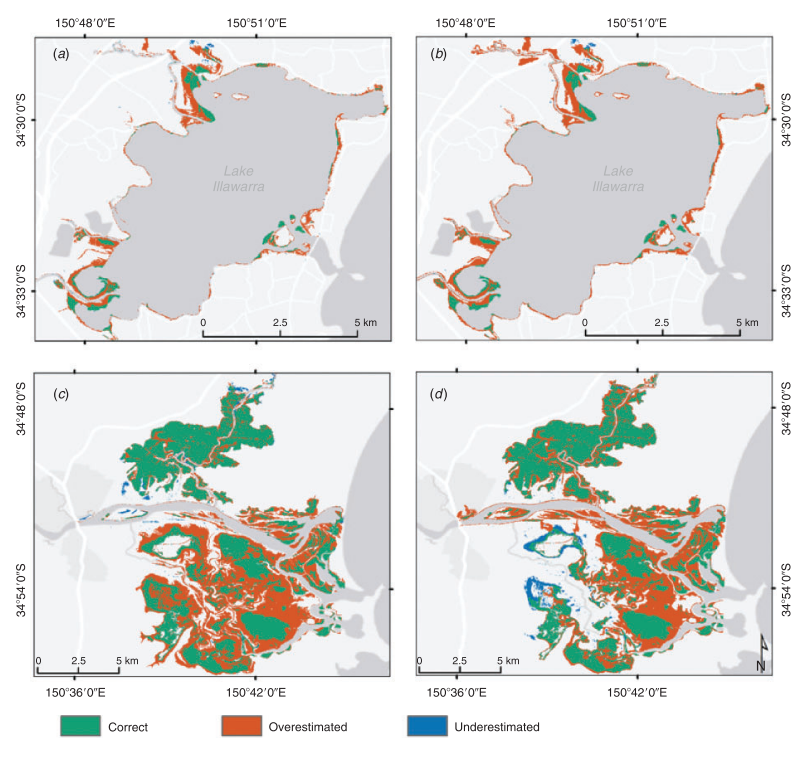
\includegraphics[width=0.65\textwidth]{Image2_Kumbier.png}
        {\hspace{-2cm} \tiny Source: Kumbier et al (2019) }
        \caption{Innondations modélisées avec un modèle statique et hydrodynamique pour 2 estuaires}
        \label{kumbier}
    \end{figure}
    
    On peut voir que pour l'estuaire fermé où le delta ne s'est pas encore remplie de sédiments les deux modèles sont semblables et d'un point de vue de facilité d'implémentation et d'aide à la décision, le modèle très simplifié semble être adéquat au premier ordre, du moins pour cet événement. Pour l'autre cas, les différences entre les zones innondables sont plus importantes. Le modèle statique surestime l'innondation tandis que le modèle dynamique le surestime à certains endroits et sous estime à d'autres.  Ces différences sont causées par le fait que le modèle statique ne prend pas en compte la rugosité du terrain. Ils concluent les caractéristique morphologique d'un estuaire qui contrôle font une différences entre les approches de modélisations. L'article suggère que la prise en compte de l'apport des rivières et de la rugosité du terrain est importante dans les estuaires où la plaine alluviale est large et avec peu de topographie. Il propose pour tester la robustesse de ces conclusions de faire des études des différences entre les méthode de modélisation avec différentes tempêtes et différents estuaires.
    
    Pour sauver du temps de calcul et permettre des simulations sur de plus longue période de temps, \cite{Skinner2015} ont fait une étude de faisabilité avec le modèle 2D simplifié lisflood pour simuler des inondations estuarienne dans l'estuaire d'Humber en Grande-Bretagne. Après la calibration, ils montrent que le modèle offre une performance semblable au modèle 3D tout en étant beaucoup plus efficace pour déterminer les hauteurs d'eau. Ils concluent que les modèles à 2 termes peuvent être utilisé dnas les estuaires où l'hydrodynamique est simple ce qui est le cas dans leur étude. 
    
    Il est interessant de noter que selon \cite{Neelz2013} la différence de temps de calcul entre un modèle hydrodynamique 2D qui résout les équation en eau peu profonde et les modèles simplifié à 2 ou 3 termes n'est pas nécéssairement importante. En effet, la formulation de l'équation dans les modèles simplifiés nécéssite un plus petit pas de temps ce qui compense en partie les gains pour chaque pas de temps. LISFLOOD serait plus rapide qu'un modèle hydrodynamique complet mais certain modèles à deux termes sont significativement plus lent.  
    
    \cite{Lee2019} montrent bien la flexibilité des modèles 2D en le couplant directement à un modèle hydrographique pour utiliser directement l'effet des précipitations dans le bassin versant sur le débit d'une rivière comme condition frontière à l'amont d'un modèle d'innondation 2D. Leur modèle permet de prendre en compte l'effet combiné de la pluie et du ruisselement. Ils notent une modification importante dans les courants et les profondeurs d'innondations et une performance accrue du modèle pour simuler avec précision le passage d'un typhon dans la baie de masan en corée. 
    
    De plus, les modèles 2D permettent des études de sensibilité à la montée des eaux du au réchauffement climatiques. \cite{Du2018} ont effectués des simulations d'estuaires idéalisés dans un modèle barotrope en 2 dimension pour montrer que la géométrie du bassin de l'estuaire avait un rôle important à jouer sur la réponse du marnage à une montée des eaux. Leurs simulation démontre que la marées est affecté par la longueur et la géométrie de la bathymétrie des estuaires. Pour les estuaires court le marnage tend à diminuer, pour les estuaires de longueur moyenne il tend à diminuer puis à augmenter et il tend à augmenter pour les estuaires plus long. Ce genre d'étude idéalisé permet de comprendre la réponse générale de différents type d'estuaire là où la modélisation hydrodynamique n'est pas possible. 
    
    Toujours sur les même deux estuaires \cite{Kumbier20182} ont utilisé les mêmes modèles hydrodynamique que dans \cite{Kumbier2019} pour faire des études de cas sur l'impact de la montée des eaux pour différente morphologie. Ils concluent quant à eux que l'élévation de la plaine innondable de l'estuaire est fondamentale pour identifier les systèmes les plus vulnérables. En effet, passé une certaine hauteur critique d'augmentation du niveau d'eau, la plaine innondable relativement basse et sans topographie de l'estuaire de shoalhaven voyait la profondeur et l'étendue de l'innondation augmenter de façon importante. Ainsi, bien qu'il ne soit pas possible de faire de modèles générales sur l'impact de la montée des eaux dèu a de nombreux effet non linéaire, la morphologie donne tout de même des indices pour identifier les endroits les plus à risque. 
    
    Pour finir, les modèles 2D permettent à la fois des études précises permettant la réalisation de cartes d'innondation qui prennent en compte de nombreux phénomènes et des études fondamentales sur la dynamique des estuaires. Il s'agit d'une stratégie de modélisation qui ne nécéssite pas trop de temps de calcul et qui est adapté pour l'hydrodynamique des estuaire à petite et à plus grande échelle. 
    
    \subsection{3D}
    
    Dans le millieu océanique, les processus baroclines prennent de l'importance et plusieurs couche en profondeurs permettent de simuler les effets de mélange et de l'appartition de pente de densité sur la côte d'où l'utilité d'un modèle 3D. \cite{Orton2012} ont constaté une diminution de la hauteur d'eau de 1 à 13 $\%$ en négligeant les variations de densité dans leur domaine 3D dans la baie de Delaware. Les effets de densité, mieux représenté en 3d, peuvent donc avoir un effet sur les innondations. Cependant leurs mise en oeuvre nécéssite des données de calibration de température et de salinité dans le domaine étudié. Il est aussi probable que ces effets soit moins important dans les petits domaines. La rivière delaware a atteint un pic de crues de 4000 $m^3/s$ et se jette dans une baie. Il s'agit de modèles nécéssitant beaucoup plus de ressources. 
    
    \cite{Yang2012} ont quant à eux montré qu'il était possible de simuler à la fois les processus d'innondation fluviales dans la plaine alluviale et la dynamique cotière de la circulation estuarienne avec un modèle 3D dont le domaine remonte le cours d'eau. Cela permet d'éviter des couplages de différents modèles et simplifie l'analyse de la dynamique de l'estuaire. 
    

    Les modèles 3D permettent de résoudre l'ensemble de l'hydrodynamique et sont des outils puissants pour les études incluant la résolution de la turbulence vertical et des effets baroclines. 
    
    
    
\section{Statistique}

    Les modèles hydrodynamiques permettent donc d'évaluer les risques d'innondation dans les estuaires et permet de simuler l'impact de différents scénarios d'innondation sur un territoire donné. Cependant, ces modèles ne permettent pas de calculer les période de retour des événements extrêmes et l'importance du lien statistiques entre les crues et les ondes de marrés. De plus, ce lien statistiques peut diminuer la période de retour d'une inondation importante \cite{Moftakhari2017,Couasnon2018}. Pour comprendre les liens statistiques entre les êvènements, il existe plusieurs méthodologie provenent des statistiques. Il est possible de simplement mesurer le nombre d'événement extrême simultané et de comparer le résultats avec des modèeles théorique indépendants. Il existe aussi des modèles statistiques qui mesurent spécifiquement la dépendance dans les extrêmes des distributions de probabilités. Ces techniques permettent de quantifier la dépendance entre deux êvenement dont les probabilité d'occurence ne sont pas indépendante. La distinction est importante car si les événement sont statistiquement dépendant il faut prendre en compte cette dépendance pour faire une évaluation des risques complète. Intuitivement, puisque les crues sont souvent causées par des précipitations et que les basses pressions accompagnant les tempêtes causes des surcôte de marées et des vagues, il est logique qu'il existe une dépendance statistique entre ces événement.
    \par
    \subsection{Delta du Rhin}
    Une étude de cas interessante pour ce genre de phénomène est le delta du Rhin. \cite{Kew2013, Klerk2015,Khanal2019} Sont trois articles qui se penche sur la dépendance entre les ondes de tempêtes et les ondes de tempêtes dans le delta du Rhin au pays bas. Dans les trois articles, les copules sont utilisés pour définir les statistiques conjointes mais différentes séries de données sont utilisés.  La méthodologie de \cite{Kew2013} est simple et prends comme données de base des proxies de la hauteur d'eau pour mesurer la dépendance statistiques entre les vents du nord nord-ouest et les précipitations reçus dans le bassin versant du Rhin. Les vents sont ainsi associé à la hauteur du niveau de la mer et la pluie à la décharge de la rivière. Pour calculer le lien statistiques, il compare le nombre d'événement conjoints mesurés c'est à dire, le nombre de jour de grand vents qui suivent un épisode de pluie intense. Il s'agit d'un approche idéalisé qui permet tout de même de trouver la distribution de probabilité des vents suite à une forte pluie et ainsi de voir si la probabilité d'une onde de tempête augmente suite à une augmentation du débit de la rivière. Il trouve qu'il existe un dépendance statistiques entre les deux variables, c'est à dire qu'il y a plus d'épisode de grand vent à la suite de  fortes pluies qu'en temps normal.
    \par
    Pour investiguer plus en détail le problème et tenter d'utiliser des indicateurs plus précis des ondes de tempêtes et du débit de la rivière que les proxies météorologiques, \cite{Klerk2015} ont utilisé des séries temporelle provenant de modèles hydrologique et hydraulique. Le modèles statistiques dans ce cas est une distribution bivarié qui mesure la corrélation mais uniquement pour les événement extrême des deux distributions de probabilités. Malgré le fait qu'ils avait des limitations au niveaux de la longueur de leurs séries temporelle (1981-2010) ils ont trouvé un lien clair entre les deux variables. Selon leur étude, un lien statistique entre les deux phénomène existe avec un décalage temporel de 6 jours entre les variables.  Ces 6 jours corespondent au temps de réponse nécéssaire pour evacuer l'excès d'eau suite à un épisode de précipitations dans le bassin versant du Rhin. Ils concluent donc que puisque la corrélation existe uniquement après 6 jours, il n'y a pas de risque suplémentaire que les deux évènement se produise de façon simultanée. Il recommande donc de ne pas prendre en compte cette dépendance dans les décisions de gestions des risques associé cours d'eau. Cependant ils n'ont pas evaluer de façon systématique les incertitude dans le modèle et l'impact de ces incetitudes sur la dépendance de la corrélation en fonction du décalage temporelle entre les séries de données.
    \par
    \cite{Khanal2019} va plus loin en utilisant des des séries temporelles de plus longues durées, des données météos forcant 2 modèles hydrologiques et un modèle d'onde de tempêtes. Ces derniers ont donc de meilleurs données permettant une analyse plus précises de la dépendance entre les deux variables. La méthodologie pour l'analyse de dépendance est la même que pour \cite{Klerk2015}. Cependant, ils concluent que le décalage de 6 jours n'est pas nécéssaire pour trouver une dépendance et que cette dernière doit être prise en compte dans une évaluation robuste des risques d'innondation dans le delta du rhin. Les auteurs mettent l'emphase sur l'importance d'utiliser des modèles physique valides dont les incertitudes sont bien comprises. De plus, ils n'ont pas pris en compte la dépendance temporelle des différents éléments de crues tel que la fonte des neige ce qui pourrait modifier les liens statistiques entre les variables.  
\par
    Il est donc interessant de noter que ces trois études trouve des résultats différents en fonction des séries de données utilisé et de la méthodologie utilisé pour le même estuaire. Cela permet de conclure qu'il est difficile de bien évaluer les risques statistiques lorsqu'on parle des événements composés. 
\par
\subsection{Copules}
    Dans la littérature récente, les copules sont devenues un outil important pour comprendre les statistiques des évênements conjoints. Les copules sont des objets mathématiques venant de la théorie des probabilités. Elles permettent de caractériser la dépendance  entre des variable aléatoire dans $\displaystyle \mathbb{R} ^{d}$ sans se préoccuper de la distribution de probabilité de ces dernières. Ce que ne permet pas les distributions bivariés classique. Les distributions bivariés classique nécéssite que les variables soit définis par la même famille de distributions univariés.\cite{genest2007} Les copules permettent entre autre de définir des outils de corrélations comme le Rho de Pearson et le Tau de Kendall qui permettent de quantifier la corrélation fonctionnelle entre les variables. Par exemple le Rho de pearson vaut -1 ou 1 lorsque deux variables sont fonctions l'une de l'autre. Contrairement au coefficient de pearson qui mesure uniquement la corélation linéaire entre 2 variables. \par
    Les copules permettent aussi de construire des modèles statistiques bivariés pour calculer des périodes de retour pour les événements conjoints. Il existe de nombreux modèles bi-varié et il faut faire des phases de test sur les données afin de trouver celui qui correspond le mieux aux données. \cite{genest2007}

     Des cartes d'innondation fluviale et côtière globale ont souvent pris en compte des distribution univariés \cite{Ward2015}. Ces distribution de hauteurs d'eau néglige les interaction fluvial-océanique, ils ne sont pas valides partout. De même, aux endroits plats et près du niveau de la mer, comme l'Amazon et plusieurs bassin du sud-est de l'Asie, les interactions peuvent faire augmenter de 0.5m les niveaux maximums annuels des rivières \cite{Ikeuchi2017}. C'est pour raffiner ces modèles globaux que des études récente comme \cite{Ward2018,Hendry2019,Wu2018,Couasnon2019} tente de mieux cartographier les risques d'événements concomitants de façon régional et global. 
    
    La 
    
Dependence was assessed using Kendall’s rank correlation coefficient and copula models. We find significant dependence for skew surge conditional on annual maximum
discharge at 22\% of the stations studied, and for discharge conditional on annual maximum skew
surge at 36\% of the stations studied. Allowing a time-lag between the two variables up to 5 days, we
find significant dependence for skew surge conditional on annual maximum discharge at 56\% of
stations, and for discharge conditional on annual maximum skew surge at 54\% of stations. Using
copula models, we show that the joint exceedance probability of events in which both the design
discharge and design sea-level are exceeded can be several magnitudes higher when the dependence is
considered, compared to when independence is assumed. We discuss several implications, showing
that flood risk assessments in these regions should correctly account for these joint exceedance
probabilities.
    
    Description de \cite{Ward2018}, \cite{Wu2018} et \cite{Couasnon2019} et \cite{Hendry2019}
    




    En résumé, les estuaire sont des millieux hydrodynamiquement complexe qui existe à différentes échelles et dont les propriétés morphologique varie. Les différentes méthodologies de modélisation existantes ont chacune leurs avantages et inconvénients. Avant de choisir un modèle il est important de comprendre les objectifs de la modélisation. Choisir le modèle le plus simple possible et être réaliste par rapport aux incertitudes et aux objectifs permet de bien comprendre les résultats et facilite l'analyse.  

    


\printbibliography
\end{document}


